
\chapter{Conclusion}
\label{cpt:conclusion}

\section{Conclusion}

\begin{figure}[ht]
    \centering
    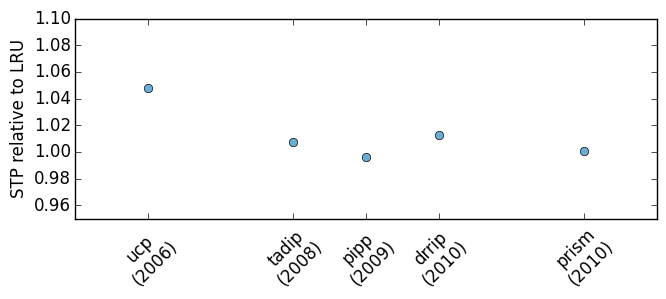
\includegraphics[width=\textwidth]{figures/results/speedup/year-comp}
    \label{fig:conclusion:yearcomp}
    \caption{Average algorithm performance measured in STP and HMS normalized to LRU by year of publication.}
\end{figure}

\todo{We have curated a list of recent and important cache partitioning algorithms}

In this thesis, we have curated a list of important and recent work in the cache management research field.
We have presented a theoretical explanation of all algorithms and compared them with each other.
A simulation framework based on Sniper was created, and several of the algorithms presented have been implemented within this framework.
We have presented some potential error sources within Sniper; most notably is the lack of precision when simulating inter-core interactions.
However, experiments were conducted to investigate the severity of this inaccuracy, and based on these results we conclude that Sniper is a viable choice for this research.

Figure~\ref{fig:conclusion:yearcomp} is a highly simplified view of our results, showing average STP and HMS for all algorithm by year, normalized to LRU performance.
Throughout our work, UCP has proven to be the best performer providing up to 5\% speedups measured in STP for our main experiment.
With constrained resources, we observed more than 20\% performance improvement with UCP.
PIPP has been unable to compete with LRU in most cases, and on average performed no better than LRU.
We suspect this is due to a short lifetime of cache blocks in a PIPP managed cache.
Both DRRIP and TADIP, which are arguably simpler schemes compared to UCP and PIPP, have shown to outperform LRU.
Neither has been able to achieve speedups comparable to UCP.
In terms of misses, we have observed that DRRIP, TADIP, and PriSM, which all attempt to reduce overall misses succeed by having as many or fewer misses than LRU.
UCP has proven to cause an increased number of misses.
While UCP is a miss minimization algorithm, it does not attempt to reduce overall misses, but rather misses caused by high utility applications.
We have shown that this causes UCP to increase the number of misses, while also improve performance.


Independent of the metric used, none of the implemented algorithms have proven to beat UCP on average.
Our results make it is tempting to conclude that UCP is the best solution.
In sections~\ref{sec:results:l3size_sensitivity} and~\ref{sec:results:bus_sensitivity} we demonstrated that changes to the simulated architecture can greatly affect algorithm performance.
While we claim that UCP is the best solution in our setup, this might not be the case in all architectural configurations.

\section{Future Work}

The time constraints put on this thesis has limited the number of algorithms presented.
Given more time we would like to continue exploring the vast research field that is cache management, and bring further algorithms into this comparison.
Implementing more algorithms within the simulation framework would also allow for more interesting results.

The Sniper simulation system has integrations to various power estimation tools.
Given that power is a concern when designing processor cores today, it would make sense to extend the simulation framework to provide power estimations as well.
With this data at hand, we would be able to use not only performance but also increased power consumption when comparing algorithms.
The potential for implementing this was not considered during this thesis, mainly because of the time constraint.
